\title{Rokko Tutorial (long version)}

% 講習会名 (例: "CMSI柏ハンズオン")
\author{11th CMSI Young Researcher Technical Workshop}

% 講習会日時(4桁-2桁-2桁. 例: "2013-04-03")
\date{4th-6th, Feb 2015}

\newcommand{\RokkoRootDir}{/opt/hands-on/rokko}
\usepackage{graphicx}
\newcommand{\smallscr}[1]{\scalebox{0.4}{$#1$}}
\newcommand{\middlescr}[1]{\scalebox{0.60}{$#1$}}

\setbeamertemplate{note page}{\insertnote\par}

\setlength{\floatsep}{5pt plus 0pt minus 0pt}                                   
\setlength{\dblfloatsep}{5pt plus 0pt minus 0pt}  % 図表と図表の間のマージン(二段組みバージョン)
\setlength{\textfloatsep}{5pt plus 0pt minus 0pt}                               
\setlength{\dbltextfloatsep}{5pt plus 0pt minus 0pt} % 図表と本文の間のマージン 
\setlength{\intextsep}{5pt plus 0pt minus 0pt}                                  
\setlength{\abovecaptionskip}{5pt plus 0pt minus 0pt}   % 図表の caption と図表本体の間のマージン
\setlength{\belowcaptionskip}{5pt plus 0pt minus 0pt}   % 図表の caption 下部のマージン

\errorcontextlines=5

\newtheorem{rei}{Example}
\renewcommand{\therei}{}

\AtBeginSection[]{
    \begin{frame}
        \tableofcontents[currentsection]
    \end{frame}
}

\begin{document}

\lstset{language=c++,basicstyle=\ttfamily\tiny,showspaces=false,keepspaces=true,rulecolor=\color[cmyk]{0, 0.29,0.84,0}}

\begin{frame}
  \titlepage
  \noindent {\footnotesize PDF file: \url{http://sf.net/projects/rokko-tutorial/files/long-tutorial-en.pdf}} \\
  \noindent {\footnotesize LaTeX source: \url{http://github.com/cmsi/rokko-tutorial/wakate}}
\end{frame}

%% \section*{Outline}
%% \begin{frame}
%%   \tableofcontents
%% \end{frame}


\section{Eigenvalue Algorithms / Solvers, Linear Algebra Libraries}


\begin{frame}
  \frametitle{Matrix diagonalization}
  \begin{itemize}
    %\setlength{\itemsep}{1em}
  \item Matrix type
    \begin{itemize}
    \item real symmetric matrix, real unsymmetric matrix, complex Hermitean matrix, complex non-Hermitean matrix
    \end{itemize}
  \item Type of matrix storage
    \begin{itemize}
      \item dense matrix, CRS (Compressed Row Storage) format, MatFree\\
            (corresponding to ``small'', ``middle'', ``large'' in TITPACK2 resp.)
    \end{itemize}
  \item Eigenvalues to be computed
    \begin{itemize}
      \item all or the greatest (least) ones in absolute value, ones in some region
    \end{itemize}
  \item Eigenvectors
    \begin{itemize}
      \item wanted/unwanted
    \end{itemize}
  \end{itemize}
\end{frame}

\begin{frame}
  \frametitle{Definitions of Terms}
  \begin{itemize}
    %\setlength{\itemsep}{1em}
  \item Eigenvalue algorithm
  \item Eigensolver (solver for eigenvalue problem)
    \begin{itemize}
      \item Implementation of eigenvalue algorithm
    \end{itemize}
  \item Eigensolver Library
    \begin{itemize}
      \item a library which consists of only eigensolvers
    \end{itemize}
  \item Linear Algebra Library
    \begin{itemize}
      \item collection of eigensolvers and other solvers
    \end{itemize}
  \item Exact diagonalization package
    \begin{itemize}
      \item Software to deal with eigenvalue problems of Hamiltonian matrix for the quantum lattice model
    \end{itemize}
  \end{itemize}
\end{frame}

\begin{frame}
  \frametitle{Eigenvalue algortihm (part)}
  \begin{itemize}
    %\setlength{\itemsep}{1em}
  \item Eigenvalue algorithms for tridiagonalized matrix
    \begin{itemize}
      \item bisection method, QR method, MR3 method, divide-conquer method+QR method
    \end{itemize}
  \item Direct diagonalization of dense matrix
    \begin{itemize}
      \item Jacobi method
    \end{itemize}
  \item Tridiagonalization of dense matrix
    \begin{itemize}
      \item Householder method
    \end{itemize}
  \item Direct diagonalization of sparse matrix
    \begin{itemize}
      \item power method, inverse power method, Rayleigh quotient iteration method, Jacobi-Davidson method, LOBPCG, Krylov-Schur method
    \end{itemize}
  \item Tridiagonalization of sparse matrix
    \begin{itemize}
      \item Lanczos method, Arnoldi method, Restart Lanczos, Thick-restart Lanczos method
    \end{itemize}
  \item Other methods
    \begin{itemize}
      \item Sakurai-Sugiura method
    \end{itemize}
  \end{itemize}
\end{frame}

\begin{frame}
  \frametitle{Eigenvalue Algothims}
  \begin{center}
    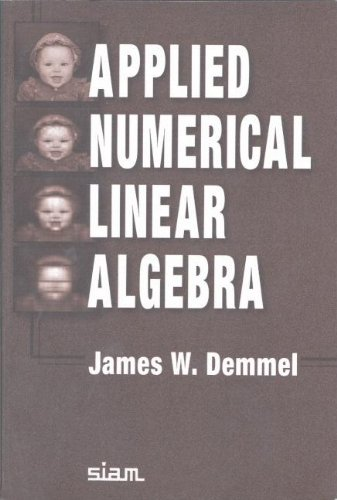
\includegraphics[height=0.45\textheight]{figure/AppliedNumericalLinearAlgebra.jpg} \ \
    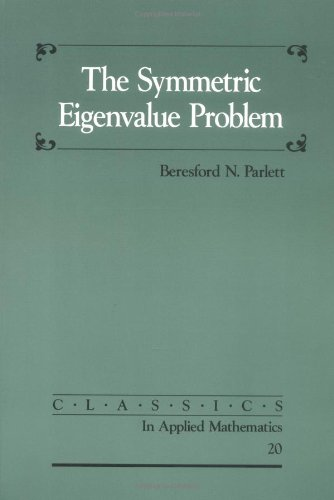
\includegraphics[height=0.45\textheight]{figure/TheSymmetricEigenvalueProblem.jpg} \ \
    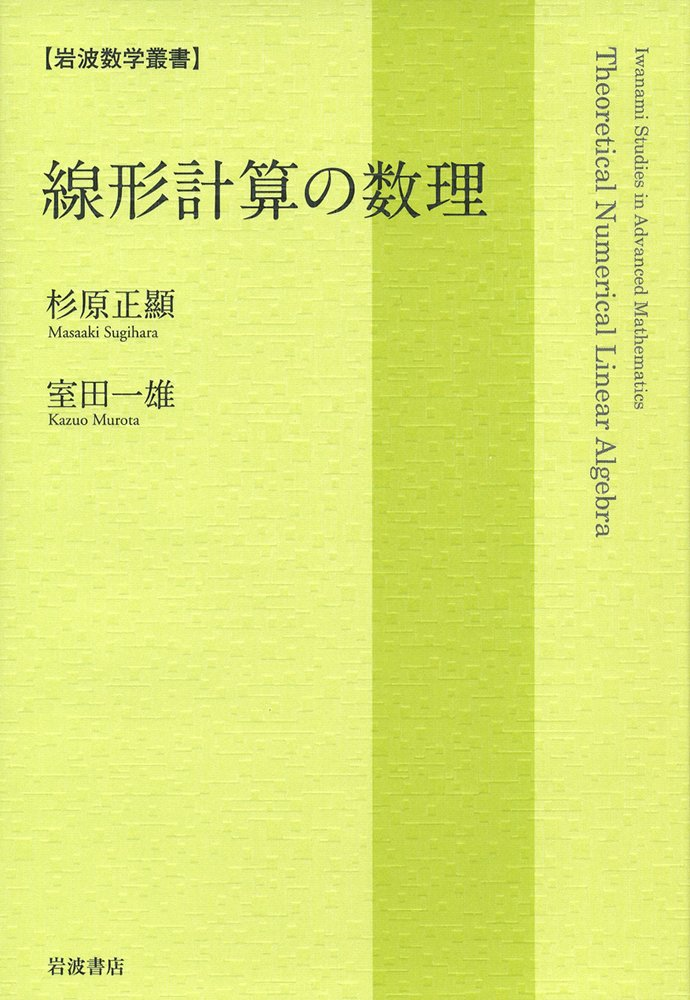
\includegraphics[height=0.45\textheight]{figure/SenkeikeisanNoSuri.jpg}  \ \
    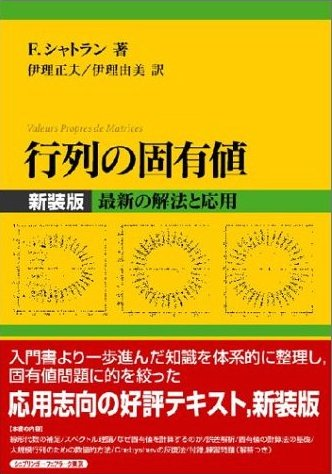
\includegraphics[height=0.45\textheight]{figure/GyoretsuNoKoyuchi.jpg}
  \end{center}
\end{frame}

\begin{frame}
  \frametitle{Existing eigesolver libraries (for dense matrix)}
  \begin{itemize}
    %\setlength{\itemsep}{1em}
  \item \href{http://www.aics.riken.jp/labs/lpnctrt/EigenExa.html}{EigenExa}: dense solver
    \begin{itemize}
      \item Householder (tri-diagonalization, penta-diagonalization) + divide\&conquer + QR
    \end{itemize}
  \item \href{http://elpa.rzg.mpg.de}{ELPA}
    \begin{itemize}
      \item Householder + divide\&conquer method + QR
    \end{itemize}
  \end{itemize}
\end{frame}

\begin{frame}
  \frametitle{Existing eigesolver libraries (for sparse matrix)}
  \begin{itemize}
  \item \href{http://trilinos.org/packages/anasazi/}{Anasazi}: Mainly iteration solvers
    \begin{itemize}
      \item Krylov-Schur, Jacobi-Davidson, XXX-Davidson, LOBPCG, Implicit Riemannian Trust Region Method
    \end{itemize}
  \item \href{http://www.caam.rice.edu/software/ARPACK/}{ARPACK}
    \begin{itemize}
      \item Implicit Restarted Lanczos
    \end{itemize}
  \item \href{https://code.google.com/p/blopex/}{BLOPEX}
    \begin{itemize}
    \item Locally Optimal Block Preconditioned Conjugate Gradient Method (LOBPCG)
    \end{itemize}
  \item \href{http://www.grycap.upv.es/slepc/}{SLEPc}: Mainly iteration solvers, Need to select seq or MPI parallel in building time
    \begin{itemize}
      \item Krylov-Schur, Generalized Davidson, Jacobi-Davidson, Rayleigh Quotient Conjugate Gradient, Contour integral Sakurai-Sugiura, Power method, Subspace Itertation, Arnoldi (explicit restart), Lanczos (explicit restart) \\
    \end{itemize}
  \item \href{http://www.comp-phys.org/software/ietl/}{IETL}: iterative solvers included in ALPS
    \begin{itemize}
      \item Lanczos, etc.
    \end{itemize}
  \end{itemize}
\end{frame}

\begin{frame}
  \frametitle{Existing linear algebra libraries (for dense matrix)}
  \begin{itemize}
    %\setlength{\itemsep}{1em}
  \item Vendor's implementation of LAPACK and ScaLAPACK
    \begin{itemize}
    \item \href{https://developer.apple.com/library/mac/documentation/Performance/Conceptual/vecLib/Reference/reference.html}{Apple VecLib}: LAPACK
    \item Fujitsu SSLII: LAPACK, a part of ScaLAPACK(part), etc.
    \item \href{https://software.intel.com/en-us/mkl_11.1_ref}{Intel MKL}: LAPACK, ScaLAPACK
    \item
      \href{http://developer.amd.com/tools-and-sdks/cpu-development/amd-core-math-library-acml/}{ACML(AMD
        Core Math Library)}: LAPACK
    \item \href{http://www.openblas.net}{OpenBLAS}: BLAS + a part of LAPACK routines (sucessive implementation for GotoBLAS)

    \end{itemize}
  \item \href{http://www.netlib.org/lapack/}{Netlib LAPACK}: Reference implementation of LAPACK
    \begin{itemize}
      \item Householder+QR, Householder + divide\&conquer + QR, Householder+bisection method, Householder+MR3
    \end{itemize}
  \item \href{http://www.netlib.org/scalapack/}{Netlib ScaLAPACK}: Reference implmentation of ScaLAPACK
    \begin{itemize}
      \item Householder + QR, Householder + divide\&conquer + QR, Householder+bisection, Householder + MR3
    \end{itemize}
  \item \href{http://eigen.tuxfamily.org/}{Eigen3}: sequential, thread parallelized for matrix-matrix product)
    \begin{itemize}
      \item Householder+QR
    \end{itemize}
%  \item \href{http://libelemental.org}{Elemental}:included eigensolvers ''MRRR'' works well, only for square processes.
%    \begin{itemize}
%      \item Householder+MR3
%    \end{itemize}
  \end{itemize}
\end{frame}

\begin{frame}
  \frametitle{Existing linear algebra libraries (for sparse matrix)}
  \begin{itemize}
    %\setlength{\itemsep}{1em}
  \item \href{http://trilinos.org}{Trilinos}: It includes eigensolvers Anasazi.
  \item Xabclib (\href{http://ppopenhpc.cc.u-tokyo.ac.jp/}{ppOpen AT})
  \end{itemize}
\end{frame}

\begin{frame}
  \frametitle{Recommnded order}
  \begin{itemize}
    %\setlength{\itemsep}{1em}
  \item For dense matrix (seq.)
    \begin{itemize}
      \item LAPACK (vendor impl.) $>$ Eigen3
    \end{itemize}
  \item For dense matrix (MPI)
    \begin{itemize}
      \item EigenExa $>$ ELPA $>$ ScaLAPACK (vendor impl.) %$>$ Elemental
    \end{itemize}
  \item For sparse matrix (seq. MPI)
    \begin{itemize}
      \item Anasazi $>$ SLEPc
    \end{itemize}
  \end{itemize}
\end{frame}

\begin{frame}
  \frametitle{Latest eigensolvers}
  \begin{itemize}
    \setlength{\itemsep}{1em}
  \item There are several hybrid-parallized(MPI+OpenMP) eigensolvers.
  \item It's almost impossible for users to implement parallel eigensolvers by themselves.
  \item Utilize open source hybrid-parallelized eigensolvers.
  \end{itemize}
\end{frame}

\begin{frame}
  \frametitle{Existing Exact diagonalization package}
  \begin{itemize}
    \setlength{\itemsep}{1em}
  \item Popular packages
    \begin{itemize}
    \item \href{http://alps.comp-phys.org/mediawiki/index.php/Main_Page}{ALPS} (\href{http://alps.comp-phys.org/static/software/applications/diag/fulldiag/doc/}{fulldiag} / \href{http://alps.comp-phys.org/mediawiki/index.php/Documentation:sparsediag}{sparsediag}): It uses LAPACK, IETL.
    \item \href{http://quattro.phys.sci.kobe-u.ac.jp/Kobe_Pack/Kobe_Pack.html}{KOBEPACK}: It includes their own eigensolvers
    \item \href{http://www-e.uni-magdeburg.de/jschulen/spin/}{SPINPACK}: It use LAPACK
    \item \href{http://www.noc.titech.ac.jp/~phys0016_nishimori/titpack2_new/index-e.html}{TITPACK2}: It includes their own eigensolvers
    \end{itemize}
  \item Sequential or thread parallelized. No MPI parallelized.
  \item It makes calculations for a large number of sites difficult.
  \end{itemize}
\end{frame}

\section{Overview and Structure of Rokko}

\begin{frame}
  \frametitle{Problems in using existing eigensolvers}
  \begin{itemize}
    \setlength{\itemsep}{1em}
  \item Different designs (interface, block size, padding...) for different eigensolvers
  \item Documentation is insufficient.
  \item Different compiling / link options depending on architectures
  \item Linking problems between languages C++ / C / Fortran
  \item Complicated dependency among lower level libraries
  \item Users want rough estimate for performace of eigensolvers before trying it.
  \end{itemize}
\end{frame}

\begin{frame}
  \frametitle{Dependency of parallel dense solvers}
  \begin{center}
    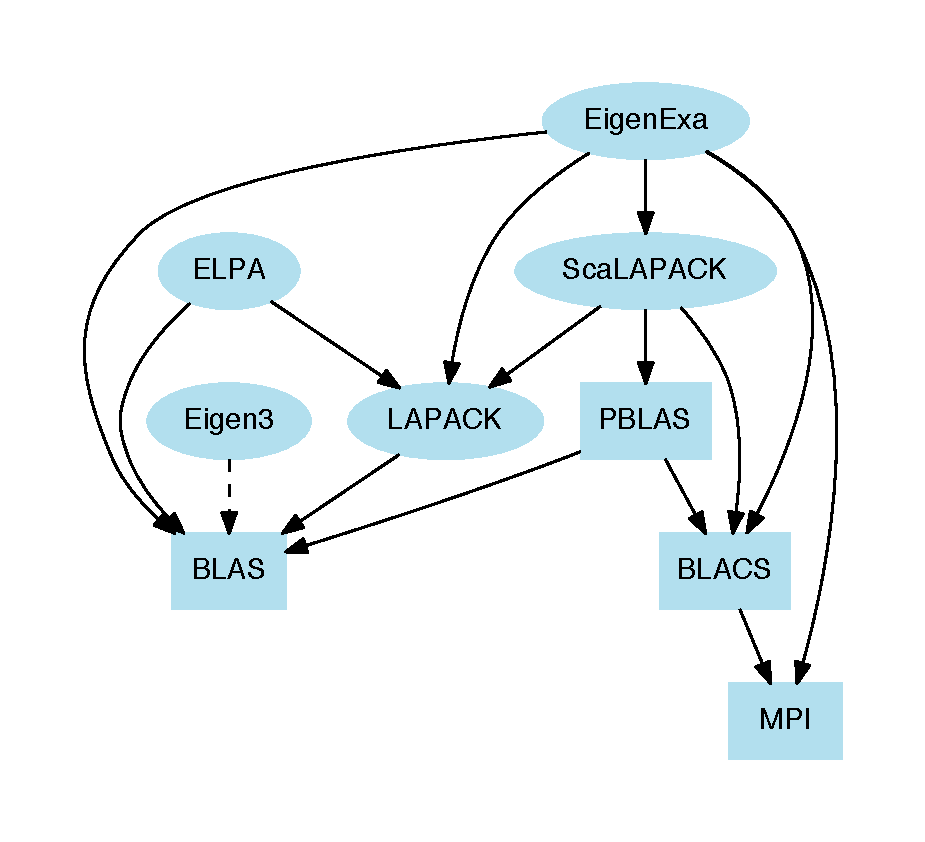
\includegraphics[height=0.8\textheight]{figure/eigensolver_dependency.pdf}
  \end{center}
\end{frame}

\begin{frame}
  \frametitle{Delvelopers of Rokko}
  \begin{itemize}
    \setlength{\itemsep}{1em}
  \item Tatsuya Sakashita (ISSP, Tokyo Univ.) \ \href{mailto:t-sakashita@issp.u-tokyo.ac.jp}{t-sakashita@issp.u-tokyo.ac.jp}
  \item Ryo Igarashi (ISSP, Tokyo Univ.) \ \href{mailto:rigarash@issp.u-tokyo.ac.jp}{rigarash@issp.u-tokyo.ac.jp}
\item Yuichi Motoyama (ISSP, Tokyo Univ.) \ \href{mailto:y-motoyama@issp.u-tokyo.ac.jp}{y-motoyama@issp.u-tokyo.ac.jp}
  \item Tsuyoshi Okubo (ISSP, Tokyo Univ.) \ \href{mailto:t-okubo@issp.u-tokyo.ac.jp}{t-okubo@issp.u-tokyo.ac.jp}
  \item Synge Todo (Department of Physics / ISSP, Tokyo Univ.) \ \href{mailto:wistaria@phys.s.u-tokyo.ac.jp}{wistaria@phys.s.u-tokyo.ac.jp}
  \end{itemize}
\end{frame}

\begin{frame}
  \frametitle{Overview of Rokko}
  \begin{itemize}
    %\setlength{\itemsep}{1em}
  \item Language
    \begin{itemize}
      %\setlength{\itemsep}{1em}
    \item Core parts: C++
    \item Language binding: C, Fortran90
    \item Benchmarking script: Python
    \end{itemize}
  \item License
    \begin{itemize}
      %\setlength{\itemsep}{1em}
    \item Boost licene (almost freely available)
    \end{itemize}
  \item Source code
    \begin{itemize}
      %\setlength{\itemsep}{1em}
    \item Open to the public by GitHub\\
          \url{https://github.com/t-sakashita/rokko/}
    \end{itemize}
  \end{itemize}
\end{frame}


\begin{frame}
  \frametitle{Design Policy of Rokko}
  \begin{itemize}
    \setlength{\itemsep}{1em}
  \item Common vector and matrix class
  \item Absorb differences of indivisual solvers by wrappers
    \begin{itemize}
      %\setlength{\itemsep}{1em}
    \item As eigensolvers develop and change, we modify wrapping functions to keep Rokko's interface the same.
    \end{itemize}
  \item Without recompiling Rokko, you can select solver in runtime.
  \item Multiple solvers can be called at one program.
  \item Less overhead wrappers by using virutal functions and templates
  \item Available from C++, C, Fortran90
  \end{itemize}
\end{frame}

\begin{frame}
  \frametitle{Components of Rokko}
  \begin{itemize}
    %\setlength{\itemsep}{1em}
  \item Install scripts for eigenvalue solvers / linear algebra libraries
  \item Common fundamental classes (distributed matrix, process grid, etc.)
  \item Wrappers for eigensolvers (in C++)
  \item Factory for eigensolvers (in C++)
  \item C/Fortran wrapper
  \item Test/sample programs
  \item Benchmark scripts (future work)
  \end{itemize}
\end{frame}



\begin{frame}[c,fragile]
  \frametitle{Directory structure of Rokko}

\dirtree{%
 .1 \RokkoFilename{}.
 .2 \RokkoFilename{rokko}
 $\cdots$ Rokko body (header \& source files).
 .2 \RokkoFilename{sample}
 $\cdots$ Sample programs in C++.
 .3
 \href{https://github.com/t-sakashita/rokko/tree/develop/sample/dense}{dense}
 $\cdots$ for dense matrix ({seq.}\&MPI).
 .3 \href{https://github.com/t-sakashita/rokko/tree/develop/sample/sparse}{sparse} $\cdots$ for sparse matrix (MPI).
 .2 \href{https://github.com/t-sakashita/rokko/tree/develop/sample_c}{sample_c} $\cdots$ Sample programs in C.
 .3 \href{https://github.com/t-sakashita/rokko/tree/develop/sample_c/dense}{dense} $\cdots$ for dense matrix ({seq.}\&MPI).
 .3
 \href{https://github.com/t-sakashita/rokko/tree/develop/sample_c/sparse}{sparse}
 $\cdots$ spapse matrix (MPI).
 .2 \href{https://github.com/t-sakashita/rokko/tree/develop/sample_fortran}{sample_fortran}
 $\cdots$ Sample programs in Fortran.
 .3 \href{https://github.com/t-sakashita/rokko/tree/develop/sample_fortran/dense}{dense} $\cdots$ for dense matrix ({seq.}\&MPI).
 .3 \href{https://github.com/t-sakashita/rokko/tree/develop/sample_fortran/sparse}{sparse} $\cdots$ for sparse matrix (MPI).
% .2
% \href{https://github.com/t-sakashita/rokko/tree/develop/test}{test}
% $\cdots$ ctest用(インストール成否の確認).
% .2 3rd-party $\cdots$ 固有値ソルバ.
 .2 \href{https://github.com/t-sakashita/rokko/tree/develop/tutorial}{tutorial} $\cdots$ Tutorial.
 .3
 \href{https://github.com/t-sakashita/rokko/tree/develop/tutorial/titpack}{titpack}
 $\cdots$ Gradually rewriting TITPACK2 to use Rokko.
}

\end{frame}


\section{Parallel MPI dense eigensolvers}

\subsection{Basic concepts}

\begin{frame}
  \frametitle{2D process grid}
  \begin{itemize}
  \item Assigning MPI processes in 2-dimension
  \item Two types of majors: row-major / column-major
  \item Example: 4 processes (no. {\color{blue}0,1,2,3})
  \begin{figure}[htbp]
\begin{tabular}{cc}
\begin{minipage}{0.4\hsize}
\begin{center}
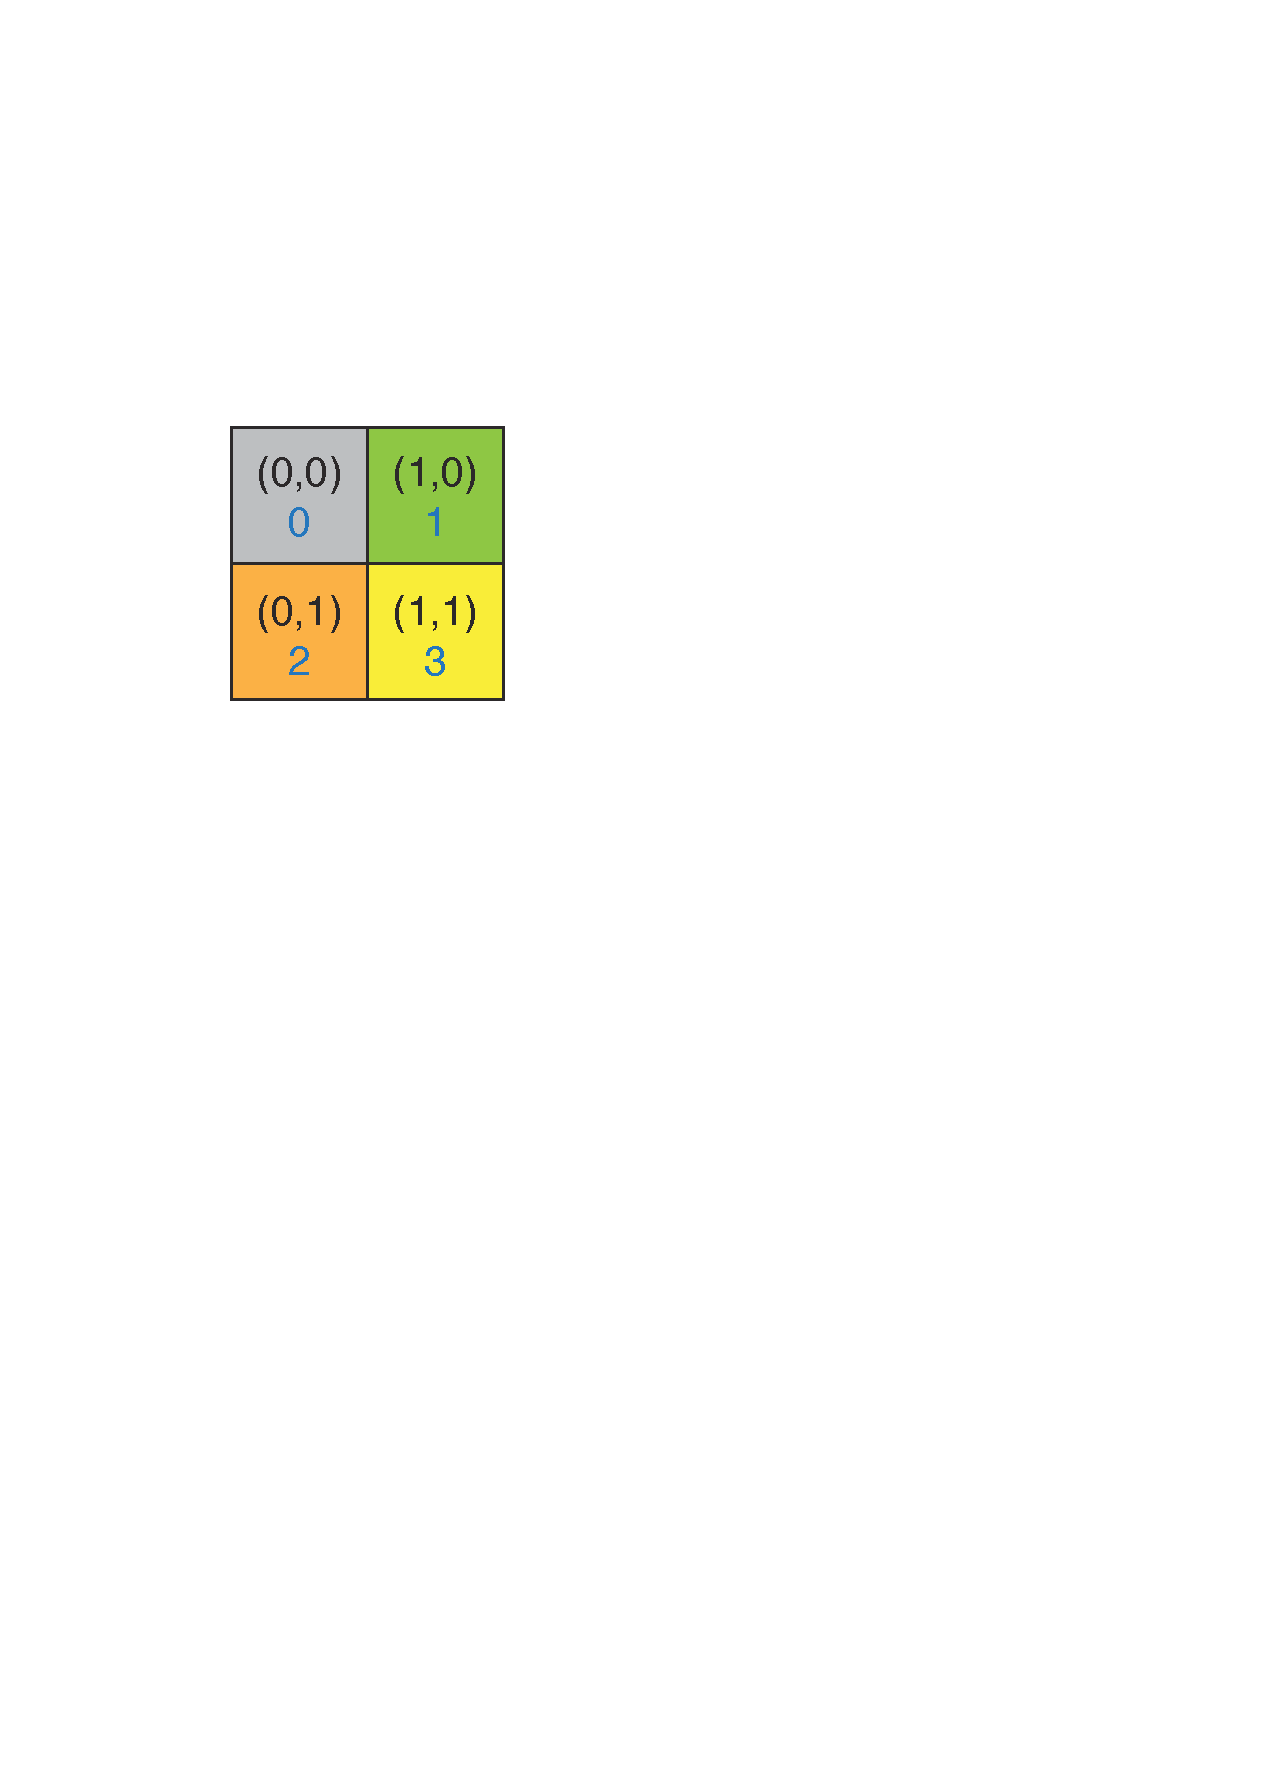
\includegraphics[height=0.25\textheight]{figure/grid-row-major.pdf}
\caption{row-major}
\label{fig:winter}
\end{center}
\end{minipage}
\begin{minipage}{0.4\hsize}
\begin{center}
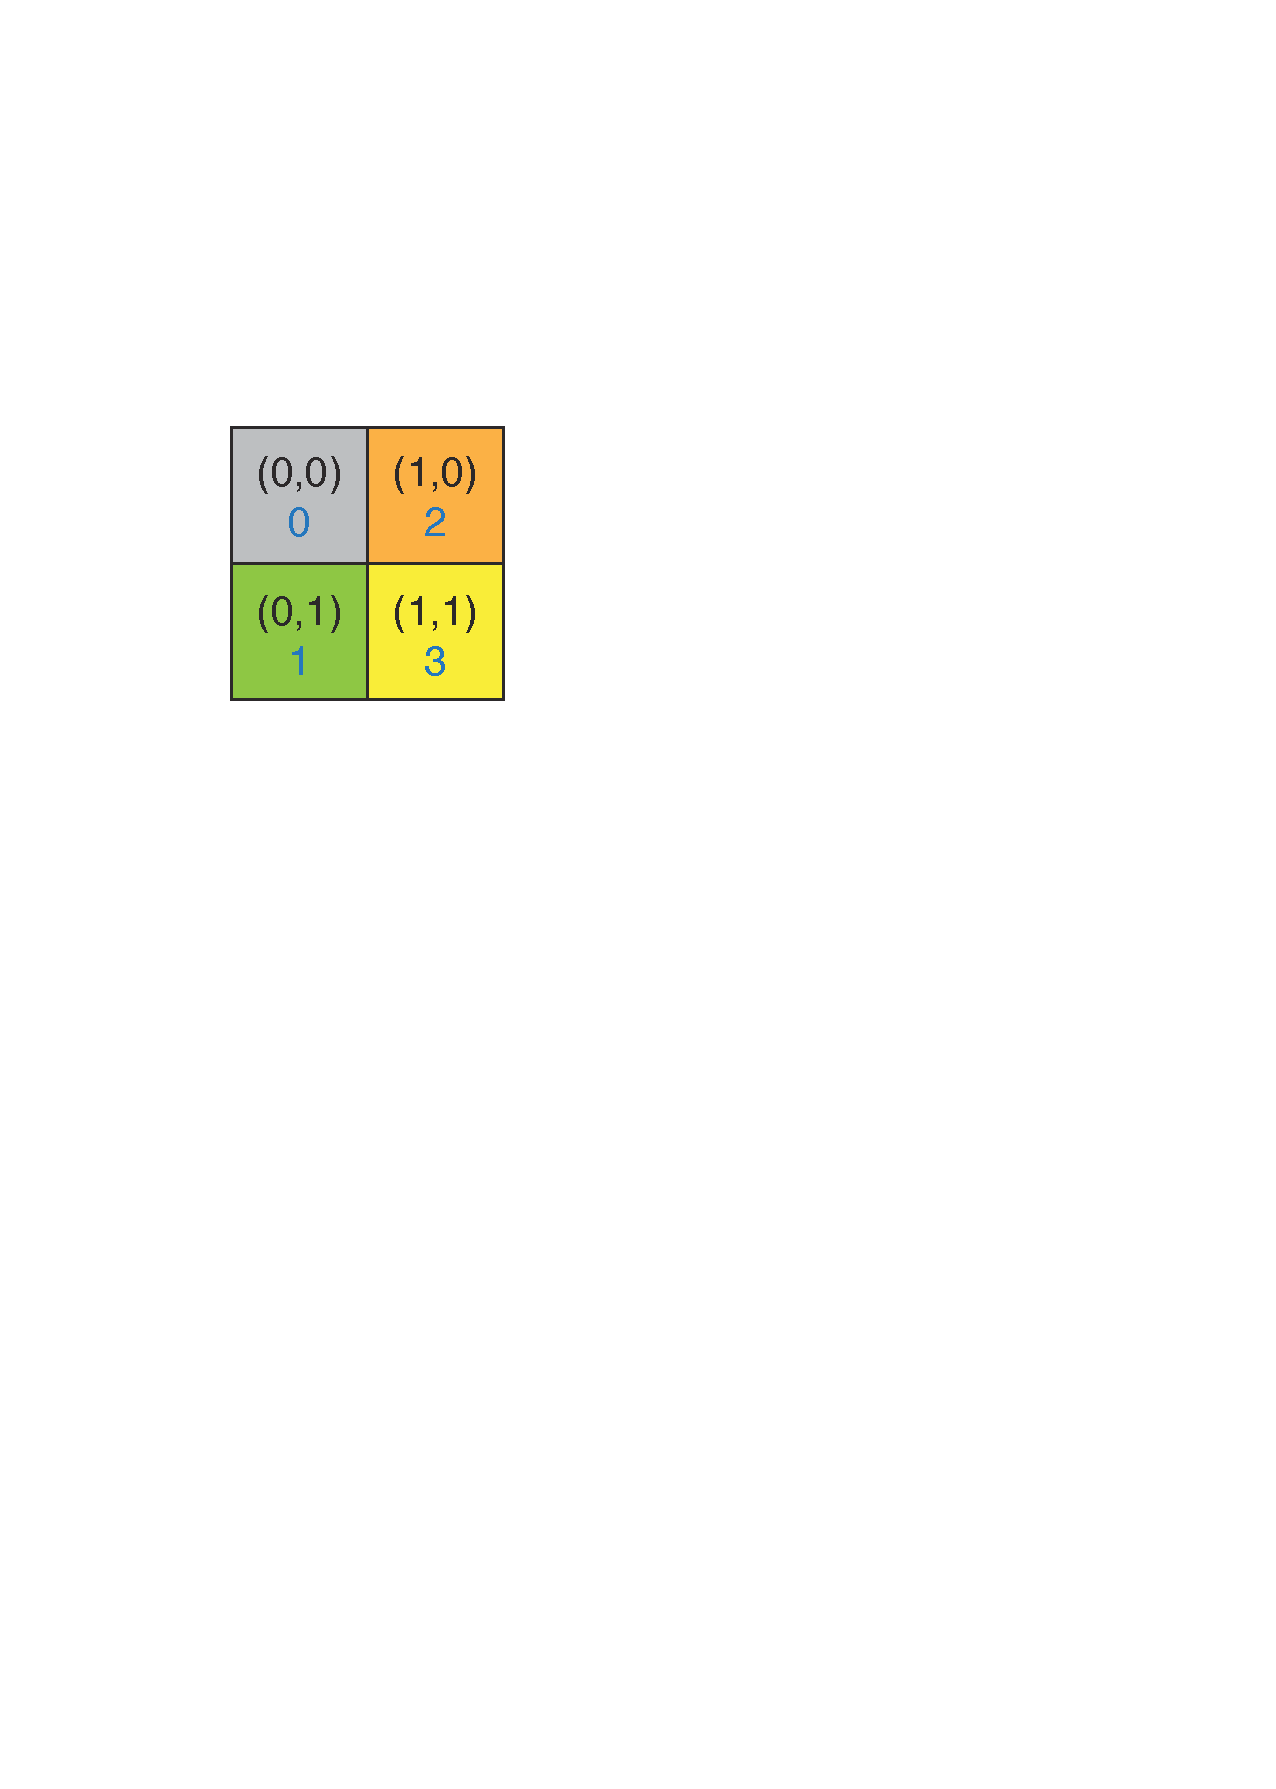
\includegraphics[height=0.25\textheight]{figure/grid-column-major.pdf}
\caption{column-major}
\label{fig:fall}
\end{center}
\end{minipage}
\end{tabular}
  \end{figure}
  \item All dense solvers support both grid majors.
  \end{itemize}
\end{frame}

\begin{frame}
  \frametitle{2-dimensional block cyclic matrix (distributed_matrix)}
  \begin{itemize}
    %\setlength{\itemsep}{1em}
  \item Parallel linear algebra libraries for dense matrices employ 2D process grid.
  \item Example (using the 2D process grid in the last page):
  \begin{figure}[htbp]
\begin{tabular}{cc}
\begin{minipage}{0.4\hsize}
\begin{center}
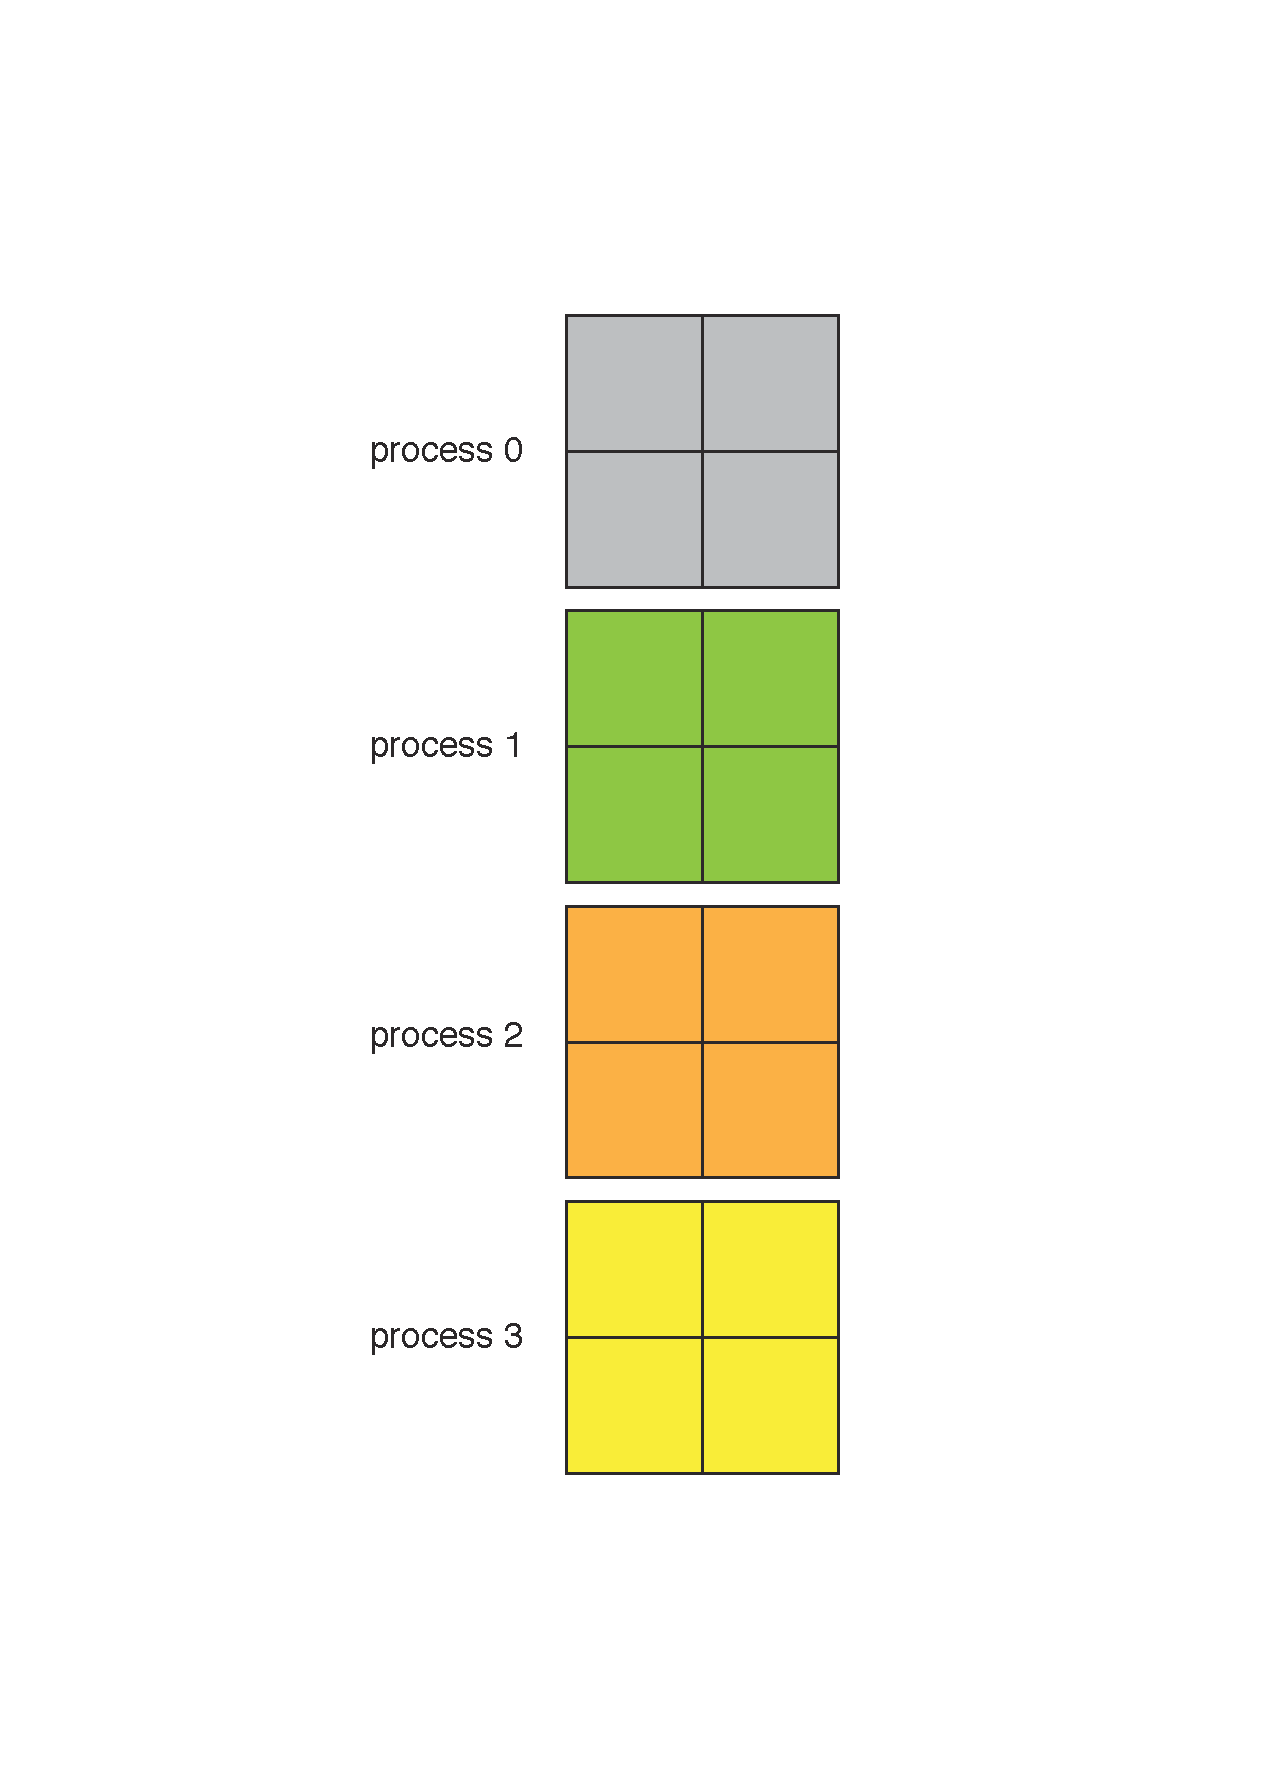
\includegraphics[height=0.45\textheight]{figure/local-view.pdf}
\caption{local view}
\label{fig:local-view}
\end{center}
\end{minipage}
\begin{minipage}{0.4\hsize}
\begin{center}
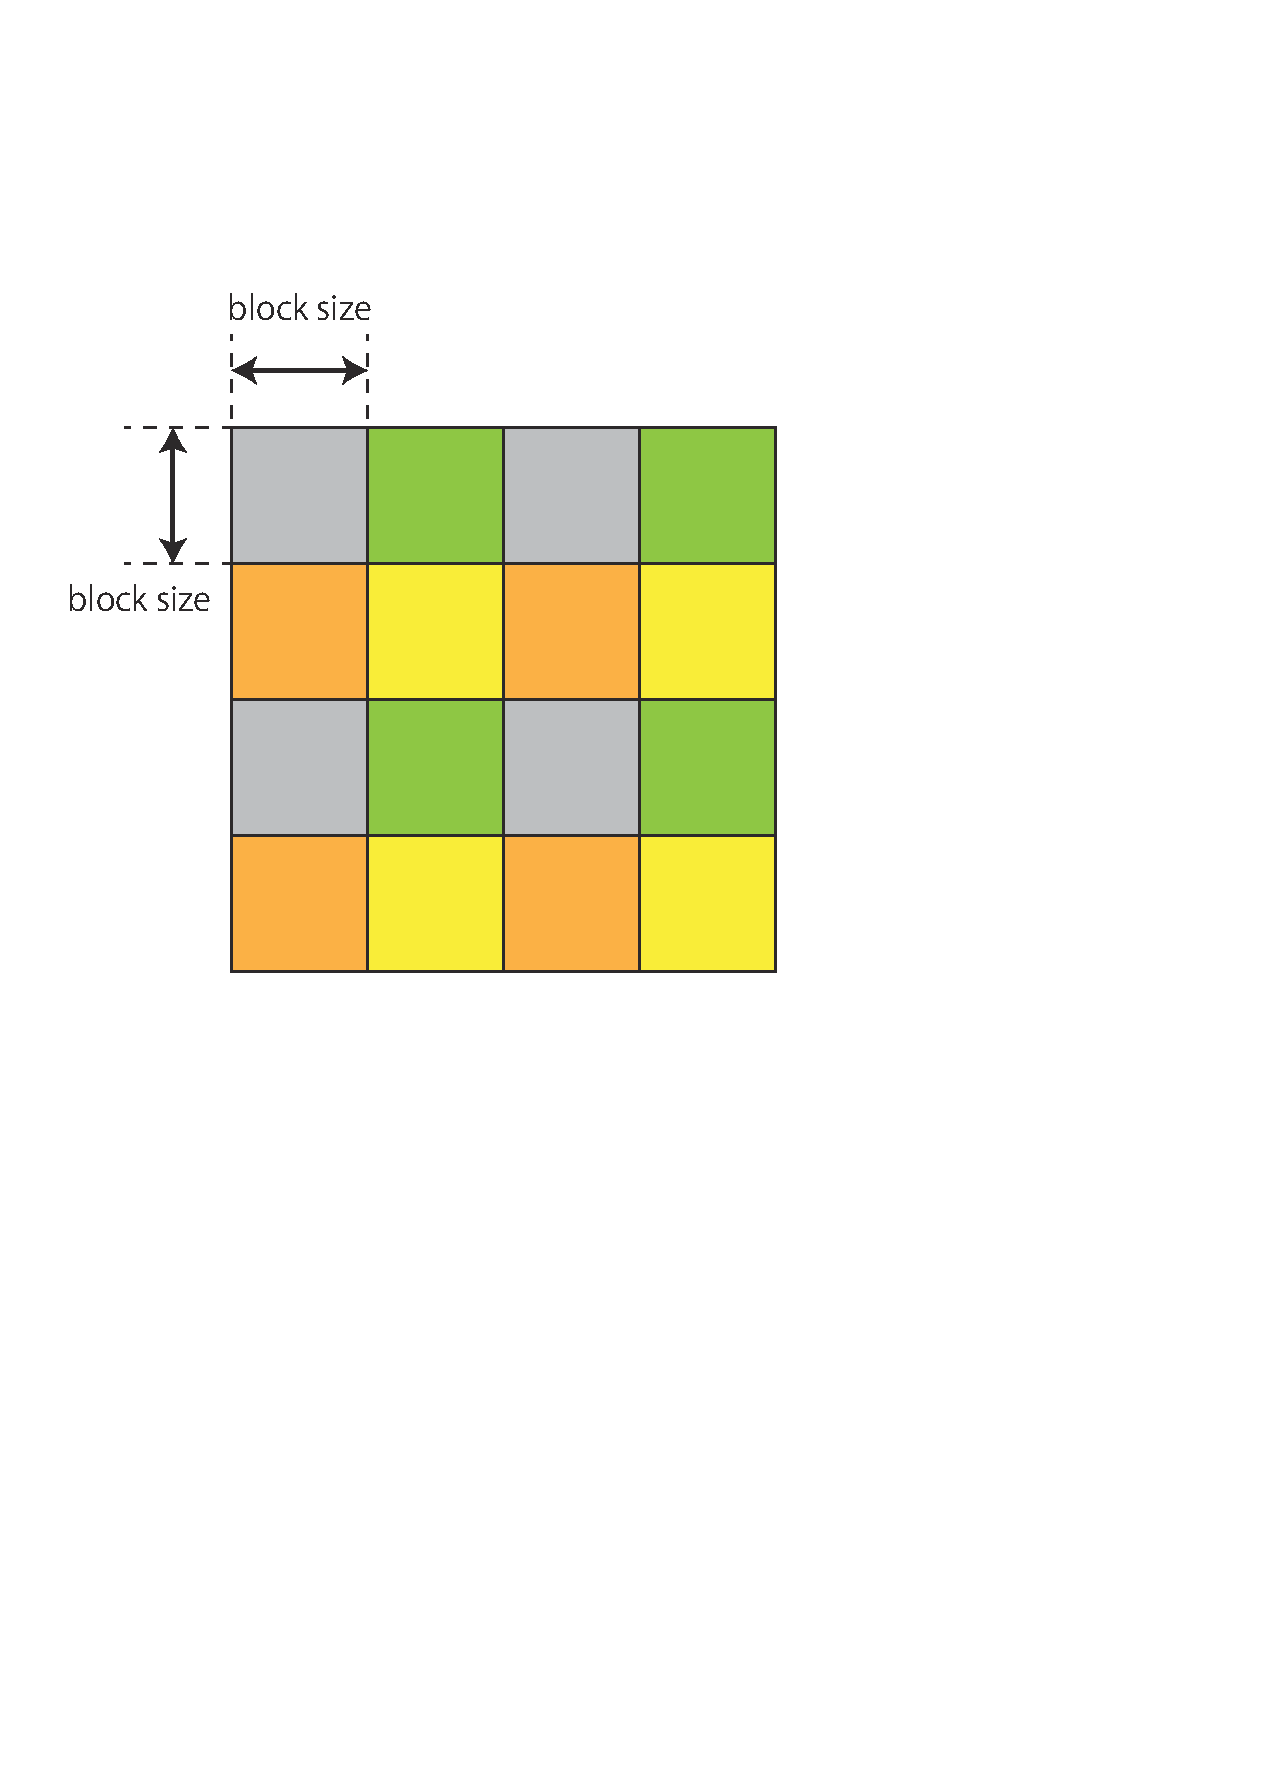
\includegraphics[height=0.45\textheight]{figure/global-view.pdf}
\caption{global view}
\label{fig:global-view}
\end{center}
\end{minipage}
\end{tabular}
  \end{figure}
  \item ScaLAPACK and ELPA support arabitrary block sizes.
  \item EigenExa support $1 \times 1$.
  \end{itemize}
\end{frame}

%% \note{%
%% As far as I know, all eigensolvers for dense matrices empoly 2D block cyclic distributed matrix.
%% Not only eigensolvers, dense linear algebra libraries (such as linear equation solver, LU / QR decomposition) use block-cyclic distribution.

%% Block-cyclic distribution is decomposed way to squared tiles according to 2D process grid defined in the last slide. 
%% Each tile is assigned to one of processes in 2D process grid.
%% The size of squared tile is called block size.
%% The colors of tiles show assigned MPI processes.

%% As an example, I use 2D process grid appeared in the previous page.
%% Paving the whole matrix with the patterns of 2D process grids of given block size, you obtain block cyclic distribution.
%% It’s virtual global view.

%% Actual local storage is obtained by pulling out the same color tiles.
%% For example, the part of process 0 is obtained by pulling out the cyan-colored tiles.
%% Similarly, the part of process 1 is obtained by pulling out the green-colored tiles.

%% EigenExa support only 1x1 block size for computational efficiency.
%% }

\subsection{Specifications of Rokko interface}

\begin{frame}[c,fragile]
  \frametitle{rokko::grid class}
  \begin{itemize}
  \item \RokkoFilename{rokko/grid.hpp}
\begin{lstlisting}
namespace rokko {
extern struct grid_row_major_t {} grid_row_major;
extern struct grid_col_major_t {} grid_col_major;
class grid {
public:
  explicit grid(MPI_Comm comm_in = MPI_COMM_WORLD);
  template <typename GRID_MAJOR>
  grid(MPI_Comm comm_in, GRID_MAJOR const& grid_major);
  MPI_Comm get_comm() const { return comm; }
  int get_nprocs() const;
  int get_nprow() const;
  int get_npcol() const;
  int get_myrank() const;
  int get_myrow() const;
  int get_mycol() const;
  bool is_row_major() const;
  bool is_col_major() const;
  int calculate_grid_row(int proc_rank) const;
  int calculate_grid_col(int proc_rank) const;
};
}
\end{lstlisting}
  \end{itemize}
\end{frame}


\begin{frame}[c,fragile]
  \frametitle{rokko::distributed_matrix class template}
  \begin{itemize}
  \item \RokkoFilename{rokko/distributed_matrix.hpp}
\begin{lstlisting}
namespace rokko {
template<typename MATRIX_MAJOR = rokko::matrix_row_major>
class distributed_matrix {
public:
  template<typename SOLVER>
  distributed_matrix(int m_global_in, int n_global_in, const grid& g_in, SOLVER const& solver_in);
  template<typename SOLVER>
  void initialize(int m_global_in, int n_global_in, const grid& g_in, SOLVER const& solver_in);
  int get_mb() const;
  int get_nb() const;
  int get_nprow() const;
  ...
  bool is_gindex_myrow(const int& global_i) const;
  bool is_gindex_mycol(const int& global_j) const;
  bool is_gindex(const int& global_i, const int& global_j) const;
  void set_local(int local_i, int local_j, double value);
  double get_local(int local_i, int local_j) const;
  void update_local(int local_i, int local_j, double value);
  void set_global(int global_i, int global_j, double value);
  double get_global(int global_i, int global_j) const;
};
}
\end{lstlisting}
  \end{itemize}
\end{frame}

\begin{frame}[c,fragile]
  \frametitle{Operation for distributed_matrix}
  \begin{itemize}
  \item Matrix-matrix product $C = \alpha A B + \beta C$
\begin{lstlisting}
  ...
  rokko::distributed_matrix<rokko::matrix_col_major> matA(dim, dim, g, solver);
  rokko::distributed_matrix<rokko::matrix_col_major> matB(dim, dim, g, solver);
  rokko::distributed_matrix<rokko::matrix_col_major> matC(dim, dim, g, solver);
  ...
  rokko::product(alpha, matA, transA, matB, transB, beta, matC);
\end{lstlisting}
  \item Scatter \& Gather for distributed_matrix
\begin{lstlisting}
  rokko::localized_matrix<LOC_MAT_MAJOR> lmat(dim, dim);
  rokko::distributed_matrix<DIST_MAT_MAJOR> mat(dim, dim, g, solver);
  rokko::scatter(lmat, mat, root);
  rokko::gather(mat, lmat, root);
\end{lstlisting}
  \end{itemize}
\end{frame}

\begin{frame}[c,fragile]
  \frametitle{generating distributed_matrix}
  \begin{itemize}
  \item Assign matrix elements (global indices)
\begin{lstlisting}
for(int global_i=0; global_i < mat.m_global; ++global_i) {
  for(int global_j=0; global_j < mat.n_global; ++global_j) {
    mat.set_global(global_i, global_j, f(global_i, global_j));
  }
}
\end{lstlisting}
  \item Assign matrix elements (local indices)
\begin{lstlisting}
for(int local_i = 0; local_i < mat.get_m_local(); ++local_i) {
  for(int local_j = 0; local_j < mat.get_n_local(); ++local_j) {
    int global_i = mat.translate_l2g_row(local_i);
    int global_j = mat.translate_l2g_col(local_j);
    mat.set_local(local_i, local_j, f(global_i, global_j));
  }
}
\end{lstlisting}
%  \item generate all matrix elements by function
%\begin{lstlisting}
%mat.generate(f);
%\end{lstlisting}
  \end{itemize}
\end{frame}

\begin{frame}[c,fragile]
  \frametitle{rokko::parallel_dense_solver class}
  \begin{itemize}
  \item Initialize solver
\begin{lstlisting}
rokko::parallel_dense_solver solver(name);
solver.initialize(argc, argv);
\end{lstlisting}
  \item Finalize solver
\begin{lstlisting}
solver.finalize();
\end{lstlisting}
  \item Diagonalize a matrix (the matrix is overwrriten)
\begin{lstlisting}
rokko::distributed_matrix<matrix_col_major> mat(dim, dim, g, solver);
...
rokko::localized_vector evals(dim);
rokko::distributed_matrix<matrix_col_major> evecs(dim, dim, g, solver);
solver.diagonalize(mat, evals, evecs);
\end{lstlisting}
%  \item 登録されているソルバの一覧
%\begin{lstlisting}
%std::vector<std::string> names = rokko::parallel_dense_solver::solvers();
%\end{lstlisting}
  \end{itemize}
\end{frame}

\subsection{Run sample}


\begin{frame}[c,fragile]
  \frametitle{Test matrix: Frank matrix (definition)}
\begin{block}{Definition}
$[a_{ij}]_{i,j = {0, \dots, n-1}} = [ n - \max(i,j) ]$\\
\end{block}

\begin{block}{Example ($n=5$)}
$[a_{ij}]_{i,j = {0, \dots, 4}} =
\begin{bmatrix}
5 & 4 & 3 & 2 & 1 \\
4 & 4 & 3 & 2 & 1 \\
3 & 3 & 3 & 2 & 1 \\
2 & 2 & 2 & 2 & 1 \\
1 & 1 & 1 & 1 & 1 \\
\end{bmatrix}
$
\end{block}
\end{frame}

\begin{frame}[c,fragile]
  \frametitle{Test matrix: Frank matrix (properties)}
\begin{block}{Analytical eigenvalues}%
$\lambda_k = \dfrac{1}{2 \left( 1 - \cos{\tfrac{2 k + 1}{2 n + 1}\pi} \right)} \quad (k=0,\dots,n-1)$
\end{block}

\begin{block}{Remark}%
Frank matrix has an eigenvalue $1$\\
\quad $\Longleftrightarrow$ $\tfrac{2 k + 1}{2 n + 1} = \tfrac{1}{3}$\\
\quad $\Longleftrightarrow$ $n-1$ is a multiple of 3.
\end{block}
\end{frame}


\begin{frame}[c,fragile]
  \frametitle{Sample program for Frank matrix (dense matrix, MPI)}

  \begin{itemize}
    \item Preperation
\begin{lstlisting}[style=shstyle]
source /opt/MateriApps/env.sh
source /opt/MateriApps/rokko/rokkoenv.sh
\end{lstlisting}
    \item Source file: \RokkoFilename{sample/dense/frank_mpi.cpp}
    \item Command to run
\begin{lstlisting}[style=shstyle]
mpirun -np 4 ./sample/dense/frank_mpi eigen_exa_sx 10
\end{lstlisting}
    \begin{itemize}
    \item 1st argument: solver name ('eigen_exa_s', scalapack', 'scalapack_pdsyevd' is also available) \\
    \item 2nd argument: size of Frank matrix (The above example deals with $10\times 10$ size Frank matrix.)
    \end{itemize}
  \item Run by job script file /opt/wakate/rokko/script/frank_mpi.sh for psi.issp.u-tokyo.ac.jp
\begin{lstlisting}[style=shstyle]
cp -r /opt/wakate/rokko/script/ .
cd script
qsub frank_mpi.sh
\end{lstlisting}
  \end{itemize}
\end{frame}

\lstset{escapechar=\#}


\begin{frame}[c,fragile]
  \frametitle{Output result for Frank matrix (dense matrix, MPI)}
\setlength { \fboxrule } { 1.5pt }
\begin{lstlisting}[style=shstyle]
Eigenvalue decomposition of Frank matrix
num_procs = 4
num_threads per process = 12
solver = eigen_exa_sx
dimension = 10
largest eigenvalues: 44.766 5.0489 1.873 #\fcolorbox{red}{white}{1}# 0.6431 0.46523 0.36621 0.30798 0.27379 0.25568
residual of the largest eigenvalue/vector: |x A x - lambda| = 2.1316e-14
timer: enabled
timer: trace = disabled
timer: detailed report = disabled
timer:     1 solver::construct                                              0.000          1
timer:     2 solver::initialize                                             0.000          1
timer:     3 solver::finalize                                               0.000          1
timer:     4 diagonalize::initialize                                        0.217          1
timer:     5 diagonalize::diagonalize                                       0.961          1
timer:     6 diagonalize::finalize                                          0.000          1
timer:    10 main                                                           2.682          1
timer:    11 generate_matrix                                                0.051          1
timer:    12 output_results                                                 0.027          1
\end{lstlisting}
You can find an eigenvalue 1\\
$\longrightarrow$ The calculation result seems correct!
\end{frame}


\section{Diagonalization of Hamailtonian matrix for quantum spin system}

\begin{frame}[c,fragile]
  \frametitle{Quantum XYZ model}
\setlength{\fboxsep}{1pt}

\noindent
$\mathcal{H}
 := \sum\limits_{\middlescr{{\langle i,j \rangle}}} \left(
  J_x^{\smallscr{\langle i,j \rangle}} \, S^x_i \cdot S^x_j
+ J_y^{\smallscr{\langle i,j \rangle}} \, S^y_i \cdot S^y_j
+ J_z^{\smallscr{\langle i,j \rangle}} \, S^z_i \cdot S^z_j
\right)$

\vspace{1\baselineskip}

\noindent
$\mathcal{H}$ is written as an sum of local Hamiltonians:\\
\noindent
$\mathcal{H} =
\sum\limits_{\middlescr{\langle i,j \rangle}}  \mathcal{H}_{\smallscr{\langle i,j \rangle}}$ \\
$\text{where} \quad  H_{\smallscr{\langle i,j \rangle}} :=
\dfrac{1}{4}
\begin{bmatrix}
J_z & & & J_x-J_y \\
 & - J_z & J_x+J_y & \\
 & J_x+J_y & - J_z & \\
J_x-J_y & & & J_z
\end{bmatrix}$

\end{frame}


\begin{frame}[c,fragile]
  \frametitle{Sample program for Hamailtonian matrix of quantum XYZ model (dense matrix, MPI)}
%%   \item Heisenberg model (seq.) \RokkoFilename{sample/dense/heisenberg.cpp}
%% \begin{lstlisting}[style=shstyle]
%% ./sample/dense/heisenberg lapack
%% \end{lstlisting}
%%   \item Heisenberg model (MPI) \RokkoFilename{sample/dense/heisenberg_mpi.cpp}
%% \begin{lstlisting}[style=shstyle]
%% mpirun -np 4 ./sample/dense/heisenberg_mpi eigen_exa_sx
%% \end{lstlisting}
%%   \item XYZ model (seq.) \RokkoFilename{sample/dense/xyz.cpp}
%% \begin{lstlisting}[style=shstyle]
%% ./sample/dense/xyz_dense lapack $HOME/rokko-0.1/test/input_data/xyz_1hexagon.ip
%% \end{lstlisting}
  \begin{itemize}
  \item Preperation
\begin{lstlisting}[style=shstyle]
source /opt/MateriApps/env.sh
source /opt/MateriApps/rokko/rokkoenv.sh
\end{lstlisting}
    \item Source file: \RokkoFilename{sample/dense/xyz_mpi.cpp}
    \item Command to run
\begin{lstlisting}[style=shstyle]
mpirun -np 4 ./sample/dense/xyz_mpi eigen_exa_sx ./xyz.dat
\end{lstlisting}
    \begin{itemize}
    \item 1st argument: solver name ('eigen_exa_s', scalapack', 'scalapack_pdsyevd' is also available) \\
    \item 2nd argument: input file (ref. next slide)
    \end{itemize}
  \item Run by job script file /opt/wakate/rokko/script/xyz_mpi.sh for psi.issp.u-tokyo.ac.jp
\begin{lstlisting}[style=shstyle]
cp -r /opt/wakate/rokko/script/ .
cd script
qsub xyz_mpi.sh
\end{lstlisting}
\end{itemize}
\end{frame}


\begin{frame}[c,fragile]
  \frametitle{Input file for Hamailtonian matrix of quantum XYZ model (dense matrix, MPI)}
xyz.dat
\begin{lstlisting}[style=shstyle]
8 8    #$\longleftarrow$number of sites, number of bonds#

0 1
1 2
2 3
3 4    #$\longleftarrow$ bonds $\langle i,j \rangle$ (pairs of site numbers)#
4 5
5 6
6 7
7 0

1.0 1.0 0.0
1.0 1.0 0.0
1.0 1.0 0.0
1.0 1.0 0.0
1.0 1.0 0.0    #$\longleftarrow
J_x^{\smallscr{\langle i,j \rangle}},\, 
J_y^{\smallscr{\langle i,j \rangle}},\,
J_z^{\smallscr{\langle i,j \rangle}}
$ for each bond ${\langle i,j \rangle}$#
1.0 1.0 0.0
1.0 1.0 0.0
1.0 1.0 0.0
\end{lstlisting}
\end{frame}

\begin{frame}[c,fragile]
  \frametitle{Output result for Hamailtonian matrix of quantum XYZ model (dense matrix, MPI)}
\begin{lstlisting}[style=shstyle]
Eigenvalue decomposition of Frank matrix
num_procs = 4
num_threads per process = 12
solver = eigen_exa_sx
dimension = 10
largest eigenvalues: 44.766 5.0489 1.873 1 0.6431 0.46523 0.36621 0.30798 0.27379 0.25568
residual of the largest eigenvalue/vector: |x A x - lambda| = 2.1316e-14
timer: enabled
timer: trace = disabled
timer: detailed report = disabled
timer:     1 solver::construct                                              0.000          1
timer:     2 solver::initialize                                             0.000          1
timer:     3 solver::finalize                                               0.000          1
timer:     4 diagonalize::initialize                                        0.217          1
timer:     5 diagonalize::diagonalize                                       0.961          1
timer:     6 diagonalize::finalize                                          0.000          1
timer:    10 main                                                           2.682          1
timer:    11 generate_matrix                                                0.051          1
timer:    12 output_results                                                 0.027          1
\end{lstlisting}
\end{frame}

\section{Install Rokko}

\begin{frame}
  \frametitle{Required tools and libraries to install Rokko}
  \begin{itemize}
    \setlength{\itemsep}{1em}
  \item CMake: \url{http://www.cmake.org}
  \item Boost C++ Libraries: \url{http://www.boost.org}
  \item Install scripts: \url{https://github.com/wistaria/installer}
  \item Lists of installation for primary supercomputer in Japan \\
    \url{https://github.com/wistaria/installer/wiki}
  \end{itemize}
\end{frame}


\begin{frame}
  \frametitle{Building system: CMake}
  \begin{itemize}
    \setlength{\itemsep}{1em}
  \item Utility to generate Makefile.\\
  It is intended to be next-generation autoconf / automake.
    \begin{itemize}
    \item It can generate Visual C++ solution file for Windows and Xcode project file for Mac OS X.
    \end{itemize}
  \item The setting for source code is described in CMakeLists.txt
  \item It has an integrated test (CTest) and binaray distribution (CPack).
  \item Automatic detection of dependency of source files
  \item Separation of source and build directories. (It makes version control easy)
  \end{itemize}
\end{frame}


\begin{frame}
  \frametitle{Installing Third-party eigensolvers / linear algebra libraries}
  \begin{itemize}
  \item Bundled packages in Rokko
    \begin{itemize}
    \item Eigen3 (This vector and matrix class is utilized in Rokko)
    \item LAPACKE (C interface of LAPACK)
    \end{itemize}
  \item Install scripts: \href{https://github.com/t-sakashita/rokko/tree/master/3rd-party/install}{3rd-party/install}
    \begin{itemize}
      \item Eigensolver libraries: Anasazi, EigenExa, ELPA, PETSc, ScaLAPACK, SLEPc
      \item Available architectures: K/FX10, x86 supercomputer/cluster (Intel compiler/GCC), Mac OS X (GCC), etc.
    \end{itemize}
  \item These solvers were already installed in psi.issp.u-tokyo.ac.jp:
/opt/MateriApps/rokko/
  \end{itemize}
\end{frame}

\begin{frame}[c,fragile]
  \frametitle{Install Rokko}
  \begin{itemize}
  \item Set environment variables (for psi.issp.u-tokyo.ac.jp)
\begin{lstlisting}[style=shstyle]
source /opt/MateriApps/env.sh
source /opt/MateriApps/rokko/rokkoenv.sh
\end{lstlisting}
  \item Copy Rokko's source code
\begin{lstlisting}[style=shstyle]
cp -r /opt/wakate/rokko/src .
\end{lstlisting}
  \item Run CMake
\begin{lstlisting}[style=shstyle]
mkdir rokko-build
cd rokko-build
\end{lstlisting}
\begin{lstlisting}[style=shstyle]
cmake -DCMAKE_CXX_COMPILER=mpicxx -DCMAKE_C_COMPILER=mpicc \
 -DCMAKE_Fortran_COMPILER=mpif90 /opt/wakate/rokko/src
\end{lstlisting}
  \end{itemize}
\end{frame}


\begin{frame}[c,fragile]
  \frametitle{Installing Rokko (cont.)}
  \begin{itemize}
  \item If you can't copy and paste the above, use the following script:
\begin{lstlisting}[style=shstyle]
bash /opt/wakate/rokko/build_script/cmake-rokko.sh
\end{lstlisting}
  \item Make, test, and install
\begin{lstlisting}[style=shstyle]
make -j 10
make test     #$\leftarrow$#or #'ctest'#
make install
\end{lstlisting}
  \end{itemize}
\end{frame}


\section{Sequential dense solvers}

\subsection{Specifications of Rokko interface}

\begin{frame}[c,fragile]
  \frametitle{rokko::localized\_matrix class template}
  \begin{itemize}
  \item \RokkoFilename{rokko/localized_matrix.hpp}
\begin{lstlisting}
namespace rokko {
template<typename MATRIX_MAJOR = rokko::matrix_row_major>
class localized_matrix {
public:
  typedef MATRIX_MAJOR major_type;
  localized_matrix();
  localized_matrix(int rows, int cols);
  template <typename T>
  localized_matrix(T const& other);
  template <typename T>
  matrix_type& operator=(T const& other);
  double operator[](int i, int j) const;
  double& operator[](int i, int j);
  int get_m_global() const;
  int get_n_global() const;
  int get_m_local() const;
  int get_n_local() const;
  bool is_gindex_myrow(const int& global_i) const;
};
}
\end{lstlisting}
  \end{itemize}
\end{frame}

\begin{frame}[c,fragile]
  \frametitle{Usage example of rokko::localized\_vector and rokko::localized\_matrix}
  \begin{itemize}
  \item \RokkoFilename{test/localized\_matrix.cpp}
\begin{lstlisting}
int dim = 3;
rokko::localized_matrix<> M(dim,dim);
M << 1,2,3,4,5,6,7,8,9;
double a = 5.0;
rokko::localized_vector u(dim);
u << 1,2,3;
rokko::localized_vector v(dim);
v << 4,5,6;
rokko::localized_vector w = a*u+M*v;
\end{lstlisting}
  \end{itemize}
\end{frame}

\begin{frame}[c,fragile]
  \frametitle{rokko::serial\_dense\_solver class}
  \begin{itemize}
    %\setlength{\itemsep}{1em}
  \item Initialize the solver
\begin{lstlisting}
rokko::serial_dense_solver solver(name);
solver.initialize(argc, argv);
\end{lstlisting}
  \item Finalize the solver
\begin{lstlisting}
solver.finalize();
\end{lstlisting}
  \item Diagonalize a dense matrix (the matrix will be overwritten)
\begin{lstlisting}
rokko::localized_matrix<matrix_col_major> mat(dim, dim, solver);
...
rokko::localized_vector evals(dim);
rokko::localized_matrix<matrix_col_major> evecs(dim, dim, solver);
solver.diagonalize(mat, evals, evecs);
\end{lstlisting}
%  \item 登録されているソルバの一覧
%\begin{lstlisting}
%std::vector<std::string> names = rokko::serial_dense_solver::solvers();
%\end{lstlisting}
  \end{itemize}
\end{frame}

\subsection{Sample programs}

\begin{frame}[c,fragile]
  \frametitle{Sample for diagonalization}
  \begin{itemize}
    %\setlength{\itemsep}{1em}
%  \item 逐次密行列ソルバーの一覧 \href{https://github.com/t-sakashita/rokko/blob/master/test/serial_dense_solvers.cpp}{test/serial\_dense\_solvers.cpp}
%\begin{lstlisting}[style=shstyle]
%./test/serial_dense_solvers
%\end{lstlisting}
  \item Using dsyev in LAPACK directyly \RokkoFilename{sample/dense/dsyev.cpp}
\begin{lstlisting}[style=shstyle]
./sample/dense/dsyev
\end{lstlisting}
  \item Using seq. dense solvers thorugh Rokko
  \begin{itemize}
    \item C++ ver. \RokkoFilename{sample/dense/frank.cpp}
\begin{lstlisting}[style=shstyle]
./sample/dense/frank lapack 5
\end{lstlisting}
    \item C ver. \RokkoFilename{sample_c/dense/frank.c}
\begin{lstlisting}[style=shstyle]
./sample_c/dense/frank lapack 5
\end{lstlisting}
    \item Fortran ver. \RokkoFilename{sample_c/dense/frank.f90}
\begin{lstlisting}[style=shstyle]
./sample_fortran/dense/frank lapack 5
\end{lstlisting}
    \end{itemize}
  \end{itemize}
\end{frame}

\section{Parallel MPI sparse solvers}

\subsection{Basic concepts}

\begin{frame}[c,fragile]
  \frametitle{CRS (Compressed Row Storage) format}
%疎行列の非ゼロ成分のみを求め固有値ソルバに渡す方法である.
%この方法で用いられる疎行列の代表的な格納方式には,CRS方式(Compressed Row Storage, 圧縮行格納方式)がある.
For each row, nonzero entries and their column indices are stored.

\begin{rei}%
\vspace{-2\baselineskip}
\begin{align*}
\begin{bmatrix}
7.1 & 5.2 & 0 & 0 \\
0 & 0 & 0 & 6.4 \\
0.2 & 0 & 0 & 4.3 \\
0 & 0 & 0.5 & 0
\end{bmatrix}
\end{align*}
Representation in CRS format:
\begin{itemize}
%\item 非ゼロ成分に対する行添字$= [1, 1, 2, 3, 3, 4] $
\item $nonzero\_rows = [2, 1, 2, 1]$
\item $nonzero\_cols = [1, 2, 4, 1, 4, 3]$
%\begin{bmatrix}
%1 & 2 \\
%4 \\
%1 & 4 \\
%3
%\end{bmatrix}$
\item $nonzero\_entries = [7.1, 5.2, 6.4, 0.2, 4.3, 0.5]$
\end{itemize}
\end{rei}

Parallelization can be done for rows.
This parallelization is automatically done by eigensolvers.

\end{frame}

\subsection{Specifications for Rokko interfaces}

\begin{frame}[c,fragile]
  \frametitle{rokko::distributed_crs_matrix class template}
  \begin{itemize}
  \item \RokkoFilename{rokko/distributed_crs_matrix.hpp}
\begin{lstlisting}
namespace rokko {
class distributed_crs_matrix {
public:
  template<typename SOLVER>
  distributed_crs_matrix(int row_dim, int col_dim, SOLVER& solver_in)
  void insert(int row, std::vector<int> const& cols, std::vector<double> const& values);
  void insert(int row, int col_size, int* cols, double* const values);
  void complete();
  int get_dim() const;
  int num_local_rows() const;
  int start_row() const;
  int end_row() const;
  void print() const;
};
}
\end{lstlisting}
  \end{itemize}
\end{frame}


\begin{frame}[c,fragile]
  \frametitle{rokko::distributed_crs_matrix class (example)}
\RokkoFilename{sample/sparse/distributed_crs_matrix.cpp}
\begin{lstlisting}
  rokko::parallel_sparse_solver solver("anasazi");
  int dim = 4;
  rokko::distributed_crs_matrix mat(dim, dim, solver);

  int num_nonzero_cols[] = {2, 1, 2, 1};
  int nonzero_cols[] = {0, 1, 3, 0, 3, 2};
  double values[] = {7.1, 5.2, 6.4, 0.2, 4.3, 0.5};

  int current = 0;
  for (int row = 0; row < dim; ++row) {
    mat.insert(row, num_nonzero_cols[row], &nonzero_cols[current], &values[current]);
    current += num_nonzero_cols[row];
  }
  mat.complete();
  mat.print();
\end{lstlisting}
\noindent
Run sample
  \begin{itemize}
  \item For using Anasazi
\begin{lstlisting}[style=shstyle]
mpirun -np 4 ./sample/sparse/distributed_crs_matrix anasazi
\end{lstlisting}
  \item For using SLEPc
\begin{lstlisting}[style=shstyle]
mpirun -np 4 ./sample/sparse/distributed_crs_matrix slepc
\end{lstlisting}
  \end{itemize}
\end{frame}


\begin{frame}[c,fragile]
  \frametitle{Matrix free method}
%たいていの疎行列向け固有値ソルバでは、行列そのものではなく、固有値分解を行うべき行列とベクトル積を行うルーチンのみが必要である。
% \\
%\noindent
%Write a class
  \begin{itemize}
  \item \RokkoFilename{rokko/utility/heisenberg_hamiltonian.hpp}
\begin{lstlisting}
class heisenberg_op : public rokko::distributed_mfree {
public:
  heisenberg_op(int L, const std::vector<std::pair<int, int> >& lattice) : L_(L), lattice_(lattice) {
    comm_ = MPI_COMM_WORLD;
    int nproc;
    MPI_Comm_size(comm_, &nproc);
    int n = nproc;
    int p = -1;
    do {
      n /= 2;
      ++p;
    } while (n > 0);
    local_N = 1 << (L-p);
    buffer_.assign(local_N, 0);
    dim_ = 1 << L;
  }
  void multiply(const double* x, double* y) const {
    rokko::heisenberg_hamiltonian::multiply(comm_, L_, lattice_, x, y, &(buffer_[0]));
  }
  int get_dim() const {
    return dim_;
  }
  int get_num_local_rows() const {
    return local_N;
  }
\end{lstlisting}
  \end{itemize}
\end{frame}

\begin{frame}[c,fragile]
  \frametitle{Matrix free method (cont.)}
\begin{lstlisting}
private:
  MPI_Comm comm_;
  mutable std::vector<double> buffer_;
  int L_;
  int local_N;
  std::vector<std::pair<int, int> > lattice_;
  int dim_;
};
\end{lstlisting}
\end{frame}


\begin{frame}[c,fragile]
  \frametitle{rokko::parallel_sparse_solver class}
\vspace{-1\baselineskip}
  \begin{itemize}
  \item Initialize solver
\begin{lstlisting}
rokko::parallel_sparse_solver solver(name);
solver.initialize(argc, argv);
\end{lstlisting}
  \item Finalize solver
\begin{lstlisting}
solver.finalize();
\end{lstlisting}
  \item Diagonalize a sparse matrix in CRS format
\begin{lstlisting}
rokko::distributed_crs_matrix mat(dim, dim, solver);
...
solver.diagonalize(mat, num_evals, block_size, max_iters, tol);
\end{lstlisting}
  \item Diagonalize MatFree
\begin{lstlisting}
heisenberg_op  mat(L, lattice);
solver.diagonalize(mat, num_evals, block_size, max_iters, tol);
\end{lstlisting}
  \item Retrieve the computed eigenvalues \& eigenvectors
\begin{lstlisting}
int i;
solver.eigenvalue(i);
std::vector<double> eigvec;
solver.eigenvector(i, eigvec);
\end{lstlisting}
%  \item 登録されているソルバの一覧
%\begin{lstlisting}
%std::vector<std::string> names = rokko::parallel_sparse_solver::solvers();
%\end{lstlisting}
  \end{itemize}
\end{frame}


\begin{frame}[c,fragile]
  \frametitle{Diagonalization Hamailtonian matrix for quantum spin system (sprase matrix, MPI)}
  \begin{itemize}
    %\setlength{\itemsep}{1em}
  \item Heisenberg model(CRS) \RokkoFilename{sample/sparse/heisenberg_crs_mpi.cpp}
%\href{https://github.com/t-sakashita/rokko/blob/master/sample_anasazi/heisenberg_crs_mpi.cpp}{sample/sparse/heisenberg\_crs\_mpi.cpp}
\begin{lstlisting}[style=shstyle]
mpirun -np 4 ./sample/sparse/heisenberg_crs_mpi
\end{lstlisting}
  \item Heisenberg model(MatFree) \RokkoFilename{sample/sparse/heisenberg_mfree_mpi.cpp}
\begin{lstlisting}[style=shstyle]
mpirun -np 4 ./sample/sparse/heisenberg_mfree_mpi
\end{lstlisting}
  \item XYZ model(CRS) \RokkoFilename{sample/sparse/xyz_crs_mpi.cpp}
\begin{lstlisting}[style=shstyle]
mpirun -np 4 ./sample/sparse/xyz_crs_mpi
\end{lstlisting}
  \item XYZ model(Matfree) \RokkoFilename{sample/sparse/xyz_mfree_mpi.cpp}
\begin{lstlisting}[style=shstyle]
mpirun -np 4 ./sample/sparse/xyz_mfree_mpi
\end{lstlisting}
  \end{itemize}
\end{frame}


\begin{frame}[c,fragile]
  \frametitle{Verification of Installation}
Display a list of available eigensolvers in Rokko\\
\RokkoFilename{tool/rokko_solvers.cpp}
\begin{lstlisting}[style=shstyle]
cd rokko/tool
./rokko_solvers
\end{lstlisting}

Output result
\begin{lstlisting}[style=shstyle]
[serial dense solvers]
  eigen3
  lapack
[parallel dense solvers]
  eigen_exa_s
  eigen_exa_sx
  scalapack
  scalapack_pdsyevd
[parallel sparse solvers]
  anasazi
  slepc
\end{lstlisting}

\end{frame}

\end{document}

